\documentclass{article}

\usepackage{amsmath, amsthm, amssymb, amsfonts}
\usepackage{thmtools}
\usepackage{graphicx}
\usepackage{setspace}
\usepackage{geometry}
\usepackage{float}
\usepackage{hyperref}
\usepackage[utf8]{inputenc}
\usepackage[polish]{babel}
\usepackage{framed}
\usepackage[dvipsnames]{xcolor}
\usepackage{tcolorbox}

% znaki polskie
\usepackage{polski}

% kod pythonowe
\usepackage{pythonhighlight}

% kropka po sekcji
\usepackage{titlesec}
\titlelabel{\thetitle.\quad}

% boldface przy caption ("Rysunek 1")
\usepackage[labelfont=bf]{caption}

\colorlet{LightGray}{White!90!Periwinkle}
\colorlet{LightOrange}{Orange!15}
\colorlet{LightGreen}{Green!15}

\newcommand{\HRule}[1]{\rule{\linewidth}{#1}}

\declaretheoremstyle[name=Theorem,]{thmsty}
\declaretheorem[style=thmsty,numberwithin=section]{theorem}
\tcolorboxenvironment{theorem}{colback=LightGray}

\declaretheoremstyle[name=Proposition,]{prosty}
\declaretheorem[style=prosty,numberlike=theorem]{proposition}
\tcolorboxenvironment{proposition}{colback=LightOrange}

\declaretheoremstyle[name=Principle,]{prcpsty}
\declaretheorem[style=prcpsty,numberlike=theorem]{principle}
\tcolorboxenvironment{principle}{colback=LightGreen}

\setstretch{1.2}
\geometry{
    textheight=9in,
    textwidth=5.5in,
    top=1in,
    headheight=12pt,
    headsep=25pt,
    footskip=30pt
}

% ------------------------------------------------------------------------------

\begin{document}

% ------------------------------------------------------------------------------
% Cover Page and ToC
% ------------------------------------------------------------------------------

\title{ \normalsize \textsc{}
		\\ [2.0cm]
		\HRule{1.5pt} \\
		\LARGE \textbf{\uppercase{Interpolacja funkcjami sklejanymi sześciennymi}
		\HRule{2.0pt} \\ [0.6cm]  \vspace*{10\baselineskip}}
		}
\date{}
\author{
        Ksawery Smoczyński \\
        Paulina Mrozińska \\
        Wojciech Pachowiak
        }



\maketitle
\newpage

\tableofcontents
\newpage

% ------------------------------------------------------------------------------

\section{Interpolujące funkcje sklejane stopnia k}
\label{sekcja1:wstęp}
Poniższa praca będzie miała na celu przybliżenie zagadnienia interpolujących funkcji 
sklejanych stopnia k. W pierwszej sekcji - \nameref{sekcja2:definicja} przedstawiona zostanie formalna definicja ww. funkcji wraz z jej postacią macierzową (\nameref
\section{Definicja}
\label{sekcja2:definicja}
\subsection{Postać macierzowa}
\label{sekcja2.1:postac_macierzowa}
\subsection{Brakujące równania}
\subsubsection{not-a-knot}
\subsubsection{natural}
\subsubsection{periodic}


\cite{kincaid_cheney}

\section{Własności numeryczne}
\textbf{\textcolor{red}{Ignorujcie na razie to co tutaj będę wrzucać. Na razie nie wiem co się dzieję, więc pojawi się tutaj wszystko i będzie to przeze mnie ciągle poprawiane, aż w końcu będzie tak jak powinno!}}


Wartość błędu bezwzględnego przybliżenia funkcji y=f(x) przez y=s(x) można
oszacować na podstawie następującej zależności:

$\mid$ f(x)-s(x) $\mid \leq \frac{7}{8} \ast {K} \ast$$ M_4$ $\ast \parallel \bigtriangleup \parallel^4$

gdzie:

$\parallel \bigtriangleup \parallel=max_{0\leq j \leq n-1}\mid x_{j+1}-x_{j}\mid$,

K=$max_{0\leq j \leq n-1} \frac{\parallel \bigtriangleup \parallel}{\mid x_{j+1}-x_j \mid }$,

$M_4=max_{0\leq j \leq n-1}\mid f^{(IV)}(x)\mid$.

 To jest link potrzebny mi chyba
 https://eia.pg.edu.pl/documents/184139/40421150/TI_LAB_5_Material_pomocniczy_b.pdf
 


https://www.cce.pk.edu.pl/~michal/pdfy/Metody16.pdf

https://wazniak.mimuw.edu.pl/index.php?title=MN11
................................................................................   To raczej tak będzie szło ...................................................

Przybliżenia generują nam błędy przybliżeń. Powstają na przykład na skutek niedoskonałości algorytmu obliczeniowego, błędów zaokrągleń,czy małej ilości danych.
Błędy przybliżenia, które możemy otrzymać przybliżając wartość za pomocą wielomianów stopnia co najwyżej trzeciego to na przykład:

Interpolacja Czebyszewa jest mniej wrażliwa na błędy zaokrągleń od
interpolacji z użyciem wzoru Lagrange'a.
Błąd interpolacji: szczególnie w przypadku, gdy liczba węzłów interpolacji jest niewystarczająca. W takim przypadku, funkcja sklejana może nie dokładnie odwzorować oryginalnej funkcji, co prowadzi do błędów interpolacji.

https://wazniak.mimuw.edu.pl/index.php?title=MN09

Błąd oscylacji: Innym problemem związanym z interpolacją funkcjami sklejanymi sześciennymi jest błąd oscylacji. Błąd ten występuje, gdy interpolowana funkcja ma duże zmiany w krótkim przedziale, co prowadzi do oscylacji funkcji sklejanej.
\begin{figure}
    \centering
    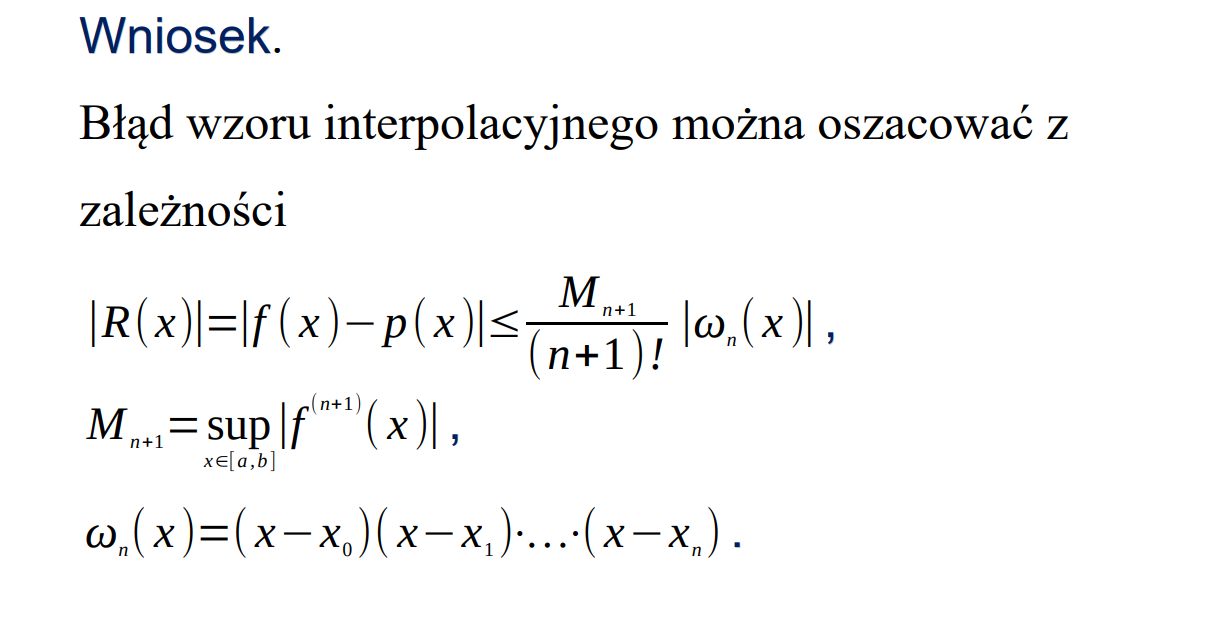
\includegraphics[width=0.5\linewidth]{image.png}
    \caption{Enter Caption}
    \label{fig:enter-label}
\end{figure}

Błąd aproksymacji: Interpolacja funkcjami sklejanymi sześciennymi może prowadzić do błędów aproksymacji, szczególnie w przypadku, gdy interpolowana funkcja jest skomplikowana lub ma wiele punktów ekstremalnych. W takim przypadku, funkcja sklejana może nie dokładnie odwzorować oryginalnej funkcji, co prowadzi do błędów aproksymacji.
\subsection{Maksymalny błąd}
\subsection{Notacja O}

Jest to notacja przedstawiająca asymptotyczne tempo wzrostu, wykorzystywana do zapisywania złożoności obliczeniowej algorytmu (miara określająca zachowanie wartości funkcji wraz ze wzrostem jej argumentów. Stosowane jest szczególnie często w teorii obliczeń, w celu opisu złożoności obliczeniowej, czyli zależności ilości potrzebnych zasobów (np. czasu lub pamięci) od rozmiaru danych wejściowych algorytmu) 


\subsection{Stabilność numeryczna}

\section{Zastosowania}
W teorii funkcje interpolacyjne sześcienne można zastosować wszędzie, gdzie mamy do dyspozycji dyskretne dane/obserwacje (tj. pary zmienna niezależna, zmienna zależna; np. w analize danych) i chcemy:
\begin{itemize}
    \item przewidzieć/zaimputować brakujące dane pośrednie poprzez nadanie im zinterpolowanych wartości (np. dla miesięcznych cen prądu, wygenerować ich dzienne ceny).
    \item móc stosować aparat matematyki ciągłej, np. liczyć pochodne lub krzywiznę bez konieczności korzystania z ich dyskretnych analogonów.
    \item zmniejszyć koszt przechowywania dużej ilości obserwacji w pamięci komputera poprzez przechowywanie tylko tych obserwacji, które posłużą za węzły interpolowane.
    \item "wygładzić" dane zaszumione lub dane o dużej wariancji poprzez, podobnie jak powyżej, potraktowanie garstki danych jako węzłów interpolacyjnych i odrzucenie reszty.
\end{itemize}

W wypadku, gdy dane/obserwacje nie są dane z góry, a zamiast tego tworzone są przez użytkownika, możemy chcieć:

\begin{itemize}
\item (w grafice komputerowej) interpolować położenia/orientacje obiektów w wirtualnym świecie, uzyskując ruch bardziej naturalny niż w wypadku prostej interpolacji liniowej.
\item komputerowo zaprojektować  meble czy samochody o gładkim/niekanciastym kształcie.
\item zaprojektować aparat ortodontyczny dopaasowany do zębów pacjenta \cite{Ahmad2012ApplicationOC}
\end{itemize} 

Jednakże w praktyce, użyteczność opisanych w tej pracy funkcji sklejanych sześciennych nie jest oczywista, biorąc pod uwagę inne funkcje sklejane, mogące wykonywać powyższe zadania równie dobrze, co funkcje sklejane sześcienne, oferując dodatkowe zalety. Przykładowo, problematyczny może być brak drobnoziarnistej kontroli nad kształtem funkcji sklejanej sześciennej - możemy manipulować jedynie położeniami jej węzłów bez możliwości określenia wartości ich  pochodnych. 
Z perspektywy projektowania odblaskowych powierzchni samochodów brak ciągłości wektorów normalmnych do krzywej wyznaczonej przez naszą funkcję sklejaną skutkuje brzydkimi odbiciami.
TODO: poprawić powyżśzej zdanie

\newpage
\section{Implementacja}

\begin{python}
from math import pi

def arctan(x,n=10):
   """Compute the mathematical value of arctan(x)

   n is the number of terms in the sum
   """
    if x < 0:
        return -arctan(-x) # recursive call
    elif x > 1: 
        return pi/2 - arctan(1/x) 
        #> (we have used that $\arctan(x)+\arctan(1/x)=\frac{\pi}{2}$ for $x>0$)
    else: 
        s = 0
        for k in range(n):
            s += (-1)**k/(2*k+1)*x**(2*k+1)
        return s 
\end{python}

\begin{figure}[htbp]
    \center
    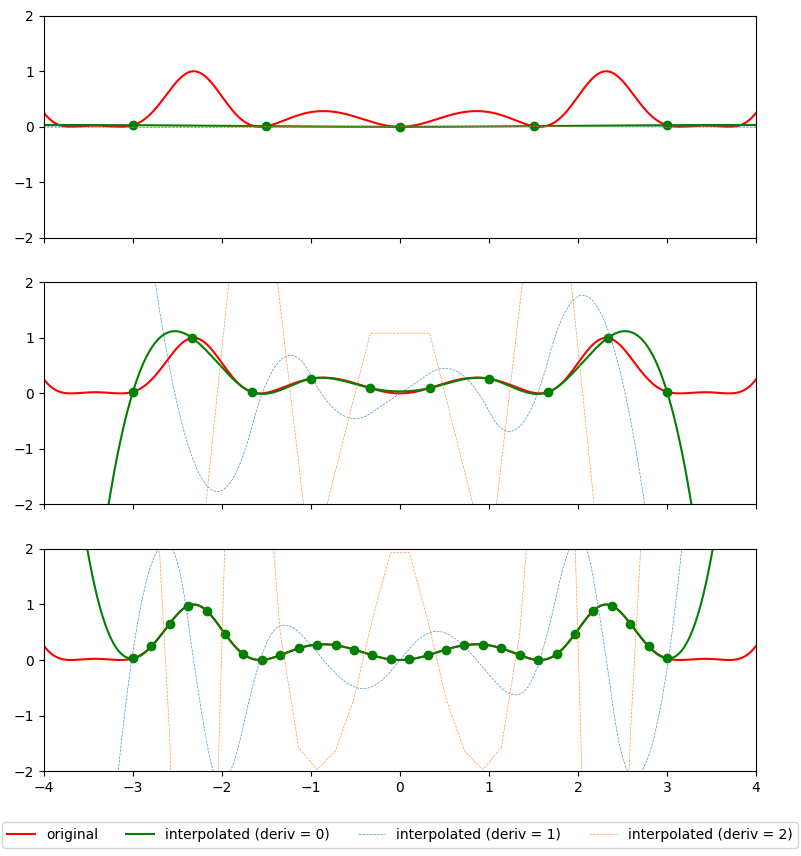
\includegraphics[width=1.0\textwidth]{plots_wide.png}
    \caption{Porównanie wykresu oryginalnej funkcji $sin(xcos(x))^2$ z wykresem funkcji interpolowanej dla 5, 10 i 30 równoodległych węzłów. Ponadto narysowane są wykresy dla 1. i 2. pochodnej funkcji interpolowanej; dla 2. pochodnej widoczne są nieróżniczkowalne "załamania" funkcji.}
\end{figure}


\newpage

% ------------------------------------------------------------------------------
% Reference and Cited Works
% ------------------------------------------------------------------------------

\bibliographystyle{apalike}
\bibliography{References.bib}


\begin{itemize}
    \item https://www.rajgunesh.com/resources/downloads/numerical/cubicsplineinterpol.pdf
    \item cheney kincaid analiza numeryczna str. ok. 330 
    \item dryja jankowscy przeglád metod i algorytmów str. ok 80
    \item https://tobydriscoll.net/fnc-julia/localapprox/splines.html
    \item numerical stability: https://math.stackexchange.com/questions/4138593/instability-of-cubic-splines
\end{itemize}


% ------------------------------------------------------------------------------

Co trzeba zrobić:
- praca pisemna w latexu (KSAWERY, WOJTEK)
- prezentowanie (to każdy umie) (PAULINA)
- kod (łatwe) (WOJTEK)
- metoda (każdy czyta) (KSAWERY pisze)
- właśnośni numeryczne (błąd przybliżenia, szybkość/ilość operacji/duże O - wybór dodawania/mnożenia, najlpeszy algorytm mnożenia macierzy) (PAULINA, WOJTEK też sprawdzi bo sie nudzi)
- zastosowania (grafika komputerowe) (WOJTEK)

SPOTKANIE 25.12

\end{document}
